% 9pt -> fonte pequena
% twocolumn -> documento em duas colunas
% extarticle -> extensão do article, classe propria para artigos/relatório
\documentclass[9pt, twocolumn]{extarticle}
\input{preâmbulo} % arquivo .tex que define vários parâmetros

% título do pdf
\title{\sffamily\bfseries
	Modelo sugerido para os relatórios\\
	e obrigatório para a documentação do projeto final
}
% autores
\author{%
	João Pedro G.C.M. Antonow	\thanks{221006351@aluno.unb.br}	\and
	Caleb Martim de Oliveira	\thanks{221017060@aluno.unb.br} 	\and
	Hiago Sousa Rocha		\thanks{221002049@aluno.unb.br} 		\and
	Luca Heringer Megiorin	\thanks{victor.lisboa@aluno.unb.br}
 \and
	Luis Augusto da Silveira Cavalcanti\thanks{victor.lisboa@aluno.unb.br}
}
% afiliação e imagem de amostra
\date{Universidade de Brasília,15 de abril de 2024\\
	\teaser{figuras/paulista1891}{Imagem de teaser (opcional)}
}

\begin{document}
	\maketitle	% imprime o título
	\abstract{% abstract/resumo do coumento
		Faça aqui uma breve descrição do que foi feito em cada seção e como elas se relacionam.
		Uma seção pode ser referenciada automaticamente usando o comando \verb|\ref{sec:label da seção}|, como mostra o texto abaixo. 
		Esse comando é usado de maneira geral para referenciar a equações, figuras, tabelas e códigos.\\
		
		\textit{``Uma dificuldade desnecessária dos alunos de OAC é o template de relatório/documentação obscuro ou altamente técnico. É o objetivo deste novo template criar um modelo mais legível e prático, e para tanto foram dedicadas três seções;
		na Seção \ref{sec:formulas}, explica-se como usar o básico das fórmulas matemáticas em \LaTeX~e como inserir figuras, tabelas e código RISC-V;
		na Seção \ref{sec:hyperlinks}, apresenta-se rapidamente como criar URLs, hyperlinks e citações a referências clicáveis;
		finalmente, na Seção~\ref{sec:casos}, são oferecidas algumas sugestões de como incluir tabelas ou figuras grandes.''}
		
		\smallskip
		\noindent
		\textbf{\sffamily Palavras-chave:} 
		OAC $\cdot$
		Assembly IRSC-V $\cdot$
		Template
	}
	
	\section{Fórmulas matemáticas}
	\label{sec:formulas}
		Uma nova seção pode ser feita simplesmente digitando \verb|\section{Nome da seção}|. 
		Esta simplicidade reaparece nas subseções e subsubseções, como veremos.
		Entretanto, antes disso, apresentemos como colocar fórmulas matemáticas; basta usar o ambiente {\tt equation}
		%
		\begin{equation}
			\label{eq:euler}
			\sum_{n=1}^\infty \frac{1}{n^2} = \frac{\pi^2}{6}
		\end{equation}
		%
		para escrever uma equação enumerada, ou o ambiente {\tt align} para múltiplas equações numeradas:
		%
		\begin{align}
			\tan(1/x) &= \frac{1}{\tan(x)} 				\label{tan1/x}	\\
			        &= \cot(x) 											\\
			        &= \tan\left(\frac{\pi}{2}-x\right) \label{pi/2-x}	\\ \implies
			      1/x &= \frac{\pi}{2}-x + 2k\pi, 		\quad k\in\mathbb{Z}.
		\end{align}	
		% 
		Repare no uso do {\tt\&} e \verb|\\| dentro do código para alinhar as equações. 
		Elas também podem ser referenciadas pelo comando \verb|\ref{}| assim como as seções, desde que você tenha criado uma label antes. Exemplo:
		
		\textit{``A equação \ref{eq:euler} é uma famosa descoberta de Leonhard Euler.''}
			
		Particularmente, equações também podem ser referenciadas por \verb|\eqref{}|:
		
		\textit{``A equação \eqref{eq:euler} é uma famosa descoberta de Leonhard Euler.''}	
		
		Para o caso do \verb|align|, é necessário criar uma \verb|\label{}| para cada equação citada.
		
		\textit{``\eqref{tan1/x} parece um problema difícil até chegarmos em \eqref{pi/2-x}.''}	
			
		Caso a numeração das equações não seja desejada, coloque {\tt equation*} e {\tt ailgn*} no lugar de {\tt equation} e {\tt align}, respectivamente.
		Finalmente, se não for desejado iniciar a fórmula em nova linha, use \verb|$$| ou \verb|\(\)| no lugar dos ambientes.\\
		Por exemplo,
		$x+y=2$ e \(\sin^2\theta+\cos^2\theta=1 \forall \theta\in\mathbb{R}\).	
		%		
			
		\subsection{Inserção de figura, tabela e código}
			Uma nova seção pode ser feita simplesmente digitando \verb|\subsection{Nome da seção}|. 
			
			Anteriormente, mostrou-se o básico do uso de matemática no \LaTeX, mas em OAC o interesse maior está em exibir figuras, tabelas, e, eventualmente, códigos RISC-V.
			
			\subsubsection{Figura}
				Colocar uma figura é bem simples:
				use o comando 
				
				\verb|\includegraphics[width=comprimento]{dir/nome}|
				
				dentro do ambiente {\tt figure}. Por exemplo,
				%
				\begin{figure}[H]\centering
					
\includegraphics[width=5cm]{figuras/logo_unb}
					\caption{legenda}
				\end{figure}
				%
				O {\tt [H]} e \verb|\centering| no código servem para fixar a posição da figura e centralizá-la, nessa ordem.
				Repare também na facilidade em escrever uma legenda através do comando \verb|\caption{}|.
				Os tipos de arquivos de imagem aceitos vão de {\tt.png}'s a {\tt.pdf}'s.
				%
			%
			
			\subsubsection{Tabela}
				O código de criação da tabela se torna tão complicada quando mais complexa for o design desejado da tabela. 
				A tabela abaixo é simples
				%
				\begin{table}[H]\centering
					\begin{tabular}{c|cccc}
						\toprule
						ISA & ALMs & Regs & MEM & DSPs \\
						\midrule
						\midrule
						RV32I   &  3271 & 1616 &     0 & 0  \\
						RV32IM  &  8070 & 1616 &     0 & 12 \\
						RV32IMF & 11341 & 4126 & 47616 & 18 \\
						\bottomrule
					\end{tabular}
					\caption{%
						Exemplo de tabela simples. 
						Repare nos símbolos dentro do código usados para alinhar as células.
					}
					\label{tab:simples}
				\end{table}
				%
				enquanto a tabela abaixo já é mais complicada.
				%
				\begin{table}[H]\centering
					\def\arraystretch{1.2} % expande a tabela
					\begin{tabular}{c|cc}
						\toprule
						\multirow{2}{*}{$n$} & 
						\multicolumn{2}{c}{$I_1$} \\
						\cline{2-3}
						& teórico & real \\ 
						\hline\hline
						40 & 14256 & 14256 \\
						50 & 22316 & 22316 \\
						60 & 32176 & 32176 \\
						70 & 43836 & 43836 \\
						80 & 57296 & 57296 \\
						90 & 72556 & 72556 \\
						100 & 89616 & 89616 \\
						\bottomrule
					\end{tabular}
					\caption{Exemplo de tabela mais complexa.}
					\label{tab:complexa}
				\end{table}
				%
				Tanto a tabela~\ref{tab:simples} quanto a~\ref{tab:complexa} foram criadas usando o ambiente {\tt tabular} dentro do ambiente {\tt table}, e em seguida definindo através de \verb|c|'s quantas colunas existem na tabela e quais delas devem ter uma linha vertical.
				Ao final, os comandos de mescla de células 
				\verb|\multirow| e \verb|\multicolumn|
				foram usados para melhorar a estética do todo.
				%
			%
			
			\subsubsection{Código RISC-V}
				Embora o grosso dos códigos relevantes aos relatórios e trabalho seja entregues em {\tt.s} ou {\tt.asm} à parte, as vezes é necessário fazer um comentário sobre um pequeno trecho, e nessa ocasião é cômodo ter o devido suporte no \LaTeX.
				
				Podemos inserir um código Assembly RISC-V no texto de duas formas:
				(i) escrevendo o código linha a linha ou 
				(ii) importanto o arquivo com o código.
				Para o primeiro caso, usa-se o ambiente {\tt lstlisting}.
				%
				\begin{lstlisting}[caption={Trecho de código Assembly RISC-V}]
				.text
				
					GameLoop:
					la	  a0, personagem
					call	Animacao
					j	    GameLoop					
					
					.include "Animacao.s"
				\end{lstlisting}
				%
				Para o segundo, usa-se o comando \verb|\lstinputlisting{dir/nome.s}|.
				%
				\lstinputlisting[caption={Código importado da pasta listings},
				                 label=listing]
				                {listings/Sleep.s}
				%
				Assim como o resto das referências até agora, você pode referenciar um listing dando \verb|\ref{}| na label apropriada. 
				
				\textit{``O listing~\ref{listing} é uma função de sleep."}
				%
			%
		%
	%
	
	\section{Hyperlinks, urls e citações}  
	\label{sec:hyperlinks}
		Até aqui, criamos hyperlinks apenas para objetos internos ao arquivo pdf.
		Em geral, podemos criar hyperlinks para páginas na web escondidos em palavras/strings ou importar URLs inteiras, assim como fazer citações do campo de bibliografia.
		
		Para introduzir uma URL, basta usar o comando \verb|\url{}|. 
		Por exempolo,
		
		\url{https://www.youtube.com}
		
		o levará para o Youtube.
		Alternativamente, você também pode utilizar o comando \verb|\href{url}{string}| para esconder o texto da URL numa palavra ou frase. 
		
		\textit{``Clique \href{https://aprender3.unb.br/login/index.php}{aqui} para entrar no aprender3."}
	          
		Por último, a listagem da sua bibliografia é convenientemente citada através do comando \verb|\cite{}|.		
				
		\textit{``Já foi demonstrado~\cite{taylor} que o erro...''}	
		
		\textit{``\cite{tipler} é um excelente livro de Física.''}						
				
	% Bibliografia -- listagem de referências		
	\begin{thebibliography}{2} % número de itens
		\bibitem{tipler} 															% nome para citação
			Mosca, Gene e Tipler, Paul A. 											% autores
			\textit{Física Volume 2, 5\textordfeminine Edição}. 					% obra/referência
			LTC--Livros Técnicos e Científicos Editora S.A., Rio de Janeiro, 2006. 	% editora, data, etc.
		
		\bibitem{taylor}												% nome para citação
			Taylor, John R.												% autores
			\textit{An Introduction to Error Analysis, Second Edition}.	% obra/referência
			University Science Books, Sausalito (CA), 1997. 			% editora, data, etc. 
	\end{thebibliography}
				
	\section{Casos especiais}	
	\label{sec:casos}
		Nem sempre é possível inserir a imagem no tamanho desejado, especialmente quando o documento se encontra, como agora, em forma de coluna dupla. 
		É claro, a mesma situação se estende para as tabelas.
		Nesses casos, considere colocar o arquivo em formato de coluna única através do comando 
		\verb|\onecolumn|, para aí colocar a(s) figura(s)/tabela(s) desejadas.
		Feito isso, retorne ao modo coluna dupla com \verb|\twocolumn|.\\
		
		\textbf{Obs.:} ambos os comandos iniciam uma página em branco.\\
		
		Se uma imagem ou tabela ocupa toda uma página, considere utilizar o ambiente {\tt sidewaysfigure} ou {\tt sidewaystable} após \verb|\onecolumn|, respectivamente.
		
		\onecolumn
		Imagens longas como a de baixo são melhor posicionadas em coluna única.
		
		\begin{figure}[H]\centering
			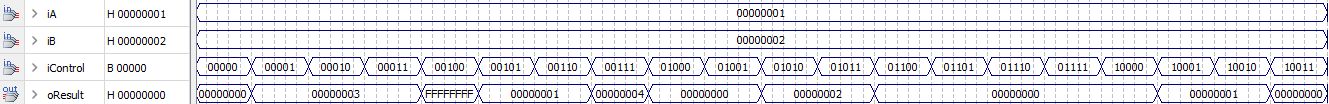
\includegraphics[width=\textwidth]
			{figuras/forma de onda.png}
			\caption{%
				Figura comprida
			}
		\end{figure}   
		
		Tabelas grandes também se beneficiam da coluna única.
		
		\begin{table}[H]\centering
			\def\arraystretch{1.2}
			\begin{tabular}{|c|c|c|}
				\hline
				Operação & Funcionalidade & Código\\
				\hline\hline
				OPAND & Faz a operação lógica AND entre dois números de 32 bits & 00000\\
				\hline
				OPOR & Faz a operação lógica OR entre dois números de 32 bits & 00001\\
				\hline
				OPXOR & Faz a operação lógica XOR entre dois números de 32 bits & 00010\\
				\hline
				OPADD & Faz a operação de soma entre dois números de 32 bits & 00011\\
				\hline
				OPSUB & Faz a operação de subtração entre dois números de 32 bits & 00100\\
				\hline
				& Põe o resultado com o valor lógico da expressão $iA < iB$, &\\
				OPSLT & isto é, se a expressão for verdadeira o resultado é um & 00101 \\
				&se for falsa o resultado é zero &\\
				\hline
				& seta o resultado com o valor logico da expressão $iA < iB$ , isto é, se a expresão & \\
				OPSLTU & for verdadeira o resultado é um se for falsa o resultado é zero, & 00110\\
				& mas desconsidera o sinal dos números iA e iB &\\
				\hline
				\multirow{2}{*}{OPSLL} & Desloca os bits de iA para a esquerda em até 31 posições & 
				\multirow{2}{*}{00111}\\
				& colocando zeros nos bits novos resultantes do deslocamento &\\
				\hline
				\multirow{2}{*}{OPSRL} & Desloca os bits de iA para a direita em até 31 posições & 
				\multirow{2}{*}{01000}\\
				& colocando zeros nos bits novos resultantes do deslocamento &\\
				\hline
				\multirow{2}{*}{OPSRA}  & desloca os bits de iA para a direita em até 31 posições & \multirow{2}{*}{01001}\\
				& conservando o sinal do número que foi deslocado &\\
				\hline
				OPLUI & carrega como resultado os 32 bits de iB & 01010\\
				\hline
				\multirow{2}{*}{OPMUL} & Faz a operação de multiplicação entre dois números de 32bits & 
				\multirow{2}{*}{01011}\\
				& e pega os 32 primeiros bits resultantes da multiplicação [31:0] & \\
				\hline
				\multirow{2}{*}{OPMULH} & Faz a operação de multiplicação entre dois números de 32bits & 
				\multirow{2}{*}{01100}
				\\
				& e pega os 32 últimos bits resultantes da multiplicação [63:32] &\\
				\hline
				\multirow{2}{*}{OPMULHU} & Faz a operação de multiplicação entre dois números de 32bits & 
				\multirow{2}{*}{01101}\\
				& sem sinal e pega os 32 últimos bits resultantes da multiplicação [63:32] & \\
				\hline
				& Faz a operação de multiplicação entre dois números de 32bits &\\
				OPMULHSU & um deles com sinal e o outro sem sinal e pega os & 01110\\
				& 32 últimos bits resultantes da multiplicação [63:32] &\\
				\hline
				OPDIV & Faz a operação de divisão entre dois números de 32 bits & 01111\\
				\hline
				OPDIVU & Faz a operação de divisão entre dois números de 32 bits sem sinal & 10000\\
				\hline
				OPREM & Faz a operação de resto da divisão entre dois números de 32 bits & 10001\\
				\hline
				OPREMU & Faz a operação de resto da divisão entre dois números de 32 bits sem sinal & 10010\\
				\hline
				OPNULL & Retorna como resultado o número zero com 32 bits & 11111\\
				\hline
			\end{tabular}
			\caption{Tabela grande.}
		\end{table}
		
		Em sequência, será colocada na próxima página uma figura deitada. 
		Para iniciar nova página em branco, escreva \verb|\newpage| ou \verb|\clearpage|.
		
		\newpage
		\begin{sidewaysfigure}\centering
			\includegraphics[width=\paperwidth]
			{figuras/máquina de estados.pdf}
			\caption{%
				Figura grande. Note a mudança de {\tt width=Xcm} para {\tt paperwidth}.
			}
		\end{sidewaysfigure}
		
		
\end{document}